\documentclass{article}
\usepackage{tikz}
\usetikzlibrary{arrows.meta, positioning}

\begin{document}

\begin{figure}[h]
    \centering
    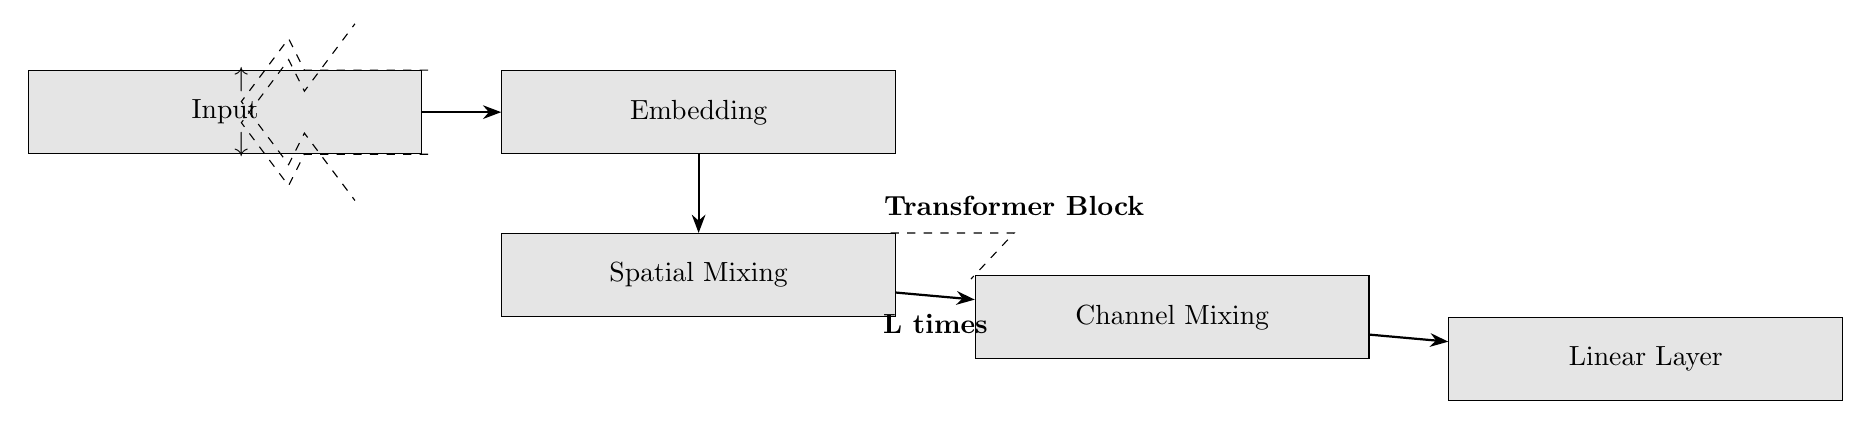
\begin{tikzpicture}[node distance=1cm, auto,
        block/.style={draw, fill=gray!20, minimum height=3em, minimum width=5cm},
        line/.style={draw, -Stealth, thick},
        transform/.style={dashed, shorten >=-2pt, shorten <=-2pt}]

        % Input
        \node[block] (input) {Input};
        
        % Embedding
        \node[block, right=of input] (embedding) {Embedding};
        
        % Spatial Mixing
        \node[block, below=of embedding.south west, anchor=north west] (spatial) {Spatial Mixing};
        \node[block, right=of spatial, anchor=north west] (channel) {Channel Mixing};
        
        % Linear Layer
        \node[block, right=of channel, anchor=north west] (linear) {Linear Layer};
        
        % Transformer Block
        \draw[transform] (spatial.north east) -- ++(1.5,0) node [above=1mm] {\textbf{Transformer Block}} -- (channel.north west);
        
        % Arrows
        \draw[line] (input) -- (embedding);
        \draw[line] (embedding) -- (spatial);
        \draw[line] (channel) -- (linear);
        \draw[line] (spatial) -- node [below=1mm] {\textbf{L times}} (channel);
        
        % Arrows to embedder
        \draw[transform] (input.north east) -- ++(-1.5,0) -- ++(-.2,.4) -- ++(-.6,-.8) node[transform, above] {$\uparrow$} -- ++(.6,-.8) -- ++(.2,.4) -- ++(.6,-.8);
        \draw[transform] (input.south east) -- ++(-1.5,0) -- ++(-.2,-.4) -- ++(-.6,.8) node[transform, below] {$\downarrow$} -- ++(.6,.8) -- ++(.2,-.4) -- ++(.6,.8);

    \end{tikzpicture}
    \caption{Overview of the used architecture based on the FourCastNet model~\cite{pathak2022fourcastnet}. We initialize the model from pre-trained weights~\cite{fcn_weights} and replace the weather-specific head with a linear head for modelling the normalized difference vegetation index (NDVI).}
    \label{fig:architecture}
\end{figure}

\end{document}